\documentclass[letterpaper]{article}
\usepackage[margin=1in]{geometry}
\usepackage[utf8]{inputenc}
\usepackage{textcomp}
\usepackage{amssymb}
\usepackage{natbib}
\usepackage{graphicx}
\usepackage{gensymb}
\usepackage{amsthm, amsmath, mathtools}
\usepackage[dvipsnames]{xcolor}
\usepackage{enumerate}
\usepackage{mdframed}
\usepackage[most]{tcolorbox}
\usepackage{csquotes}
% https://tex.stackexchange.com/questions/13506/how-to-continue-the-framed-text-box-on-multiple-pages

\tcbuselibrary{theorems}

\newcommand{\R}{\mathbb{R}}
\newcommand{\Z}{\mathbb{Z}}
\newcommand{\N}{\mathbb{N}}
\newcommand{\Q}{\mathbb{Q}}
\newcommand{\C}{\mathbb{C}}
\newcommand{\code}[1]{\texttt{#1}}
\newcommand{\mdiamond}{$\diamondsuit$}
\newcommand{\PowerSet}{\mathcal{P}}
\newcommand{\Mod}[1]{\ (\mathrm{mod}\ #1)}
\DeclareMathOperator{\lcm}{lcm}

%\newtheorem*{theorem}{Theorem}
%\newtheorem*{definition}{Definition}
%\newtheorem*{corollary}{Corollary}
%\newtheorem*{lemma}{Lemma}
\newtheorem*{proposition}{Proposition}


\newtcbtheorem[number within=section]{theorem}{Theorem}
{colback=green!5,colframe=green!35!black,fonttitle=\bfseries}{th}

\newtcbtheorem[number within=section]{definition}{Definition}
{colback=blue!5,colframe=blue!35!black,fonttitle=\bfseries}{def}

\newtcbtheorem[number within=section]{corollary}{Corollary}
{colback=yellow!5,colframe=yellow!35!black,fonttitle=\bfseries}{cor}

\newtcbtheorem[number within=section]{lemma}{Lemma}
{colback=red!5,colframe=red!35!black,fonttitle=\bfseries}{lem}

\newtcbtheorem[number within=section]{example}{Example}
{colback=white!5,colframe=white!35!black,fonttitle=\bfseries}{def}

\newtcbtheorem[number within=section]{note}{Important Note}{
        enhanced,
        sharp corners,
        attach boxed title to top left={
            xshift=-1mm,
            yshift=-5mm,
            yshifttext=-1mm
        },
        top=1.5em,
        colback=white,
        colframe=black,
        fonttitle=\bfseries,
        boxed title style={
            sharp corners,
            size=small,
            colback=red!75!black,
            colframe=red!75!black,
        } 
    }{impnote}
\usepackage[utf8]{inputenc}
\usepackage[english]{babel}
\usepackage{fancyhdr}
\usepackage[hidelinks]{hyperref}

\pagestyle{fancy}
\fancyhf{}
\rhead{CSE 131}
\chead{Friday, April 07, 2023}
\lhead{Lecture 3}
\rfoot{\thepage}

\setlength{\parindent}{0pt}

\begin{document}

\section{Introduction to Binary Operations}

\begin{mdframed}
    Consider the following s-expression: \code{(sub1 (sub1 (add1 73)))}. Looking at the code discussed in the lecture handout, and assuming \code{main} runs, what does the stack and heap look like when \begin{verbatim}
        format!("mov rax, {}", *n)\end{verbatim} 
    evaluates? 

    \begin{mdframed}
        We'll take a look at the function calls of \code{compile\_expr(\&expr)}. First, note that Rust will store objects on the stack unless you allocate it on the heap. Recall, from the previous lecture, we have the AST representation 
                \begin{verbatim}
    Expr::Sub1(
        Box::new(Expr::Sub1(
            Box::new(Expr::Add1(
                Box::new(
                    Expr::Num(73)
                )
            ))
        ))
    )\end{verbatim}
        
        Our code initially calls \code{compile\_expr(\&expr)}, where \code{\&expr} is a reference to the above object. Note that the outer \code{Expr::Sub1} is in the stack, but the data in each of the \code{Enum}s will be allocated in the heap. In any case, after calling the function initially, it makes a recursive call with the argument being the held data of the inner object. This repeats until we reach the end (when we have the \code{Num}). 
        \begin{center}
            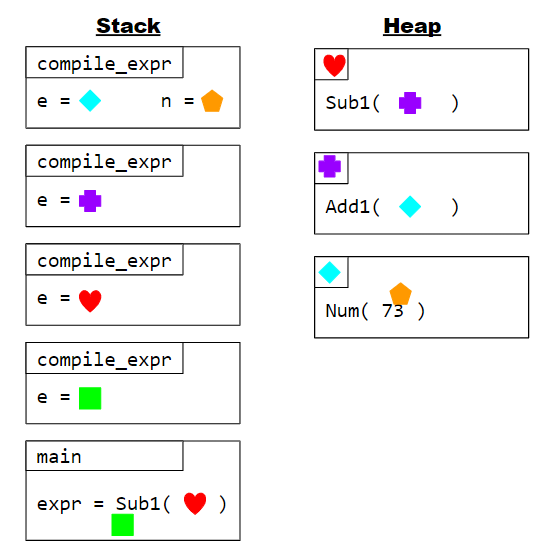
\includegraphics[scale=0.7]{../assets/memory_diagram.png}
        \end{center}
    \end{mdframed}
\end{mdframed}

\subsection{Adding Binary Operation Support}
Let's suppose we want to add \code{(+ <expr> <expr>)} to our compiler. Our grammar for our language might look like 
\begin{verbatim}
    (*
        expr := <number> 
            | (add1 <expr>)
            | (sub1 <expr>)
            | (+ <expr> <expr>) 
    *)\end{verbatim}
The \code{Expr} \code{enum} might look like 
\begin{verbatim}
    enum Expr {
        Num(i32),
        Add1(Box<Expr>),
        Sub1(Box<Expr>),
        Plus(Box<Expr>, Box<Expr>),
    }\end{verbatim} 
The \code{parse\_expr} function might look like 
\begin{verbatim}
pub fn parse_expr(s: &Sexp) -> Expr {
    match s {
        Sexp::Atom(I(n)) => Expr::Num(i32::try_from(*n).unwrap()),
        Sexp::List(list) => match &list[..] {
            [Sexp::Atom(S(op)), e] if op == "add1" => 
                Expr::Add1(Box::new(parse_expr(e))),
            [Sexp::Atom(S(op)), e] if op == "sub1" => 
                Expr::Sub1(Box::new(parse_expr(e))),
            [Sexp::Atom(S(op)), e] if op == "negate" => 
                Expr::Negate(Box::new(parse_expr(e))),
            [Sexp::Atom(S(op)), e1, e2] if op == "+" => {
                Expr::Add(Box::new(parse_expr(e1)), Box::new(parse_expr(e2)))
            }
            _ => panic!("parse error"),
        },
        _ => panic!("parse error"),
    }
}\end{verbatim}
Then, our \code{compile\_expr} function might look like 
\begin{verbatim}
    fn compile_expr(e: &Expr, si: i32) -> String {
        match e {
            Expr::Num(n) => format!("mov rax, {}", *n),
            Expr::Add1(subexpr) => compile_expr(subexpr) + "\nadd rax, 1",
            Expr::Sub1(subexpr) => compile_expr(subexpr) + "\nsub rax, 1",
            Expr::Plus(e1, e2) => {
                // ?
            }
        }
    }\end{verbatim}

There are two ways we can implement the \code{Plus} part of the function. 
\begin{center}
    \begin{tabular}{p{3in} | p{3in}}
        A & B \\ 
        \hline 
        \begin{verbatim}
let e1_instrs = compile_expr(e1);
let e2_instrs = compile_expr(e2);
e1_instrs + "\n mov rbx, rax"
    + e2_instrs + "\n add rax, rbx"\end{verbatim}
        & 
        \begin{verbatim}
let e1_instrs = compile_expr(e1, si);
let e2_instrs = compile_expr(e2, si + 1);
let stack_offset = si * 4;
format!("
    {e1_instrs}
    mov [rsp - {stack_offset}], rax
    {e2_instrs}
    add rax, [rsp - {stack_offset}]
")\end{verbatim}
    \end{tabular}
\end{center}

\begin{mdframed}
    (Exercise.) With option (a), what is the assembly code generated after compiling the following code? What is the result of running the assembly? 
    \begin{enumerate}[(a)]
        \item \code{(+ (+ 100 30) 4)}
        \begin{mdframed}
            \begin{verbatim}
	mov rax, 500
	mov rbx, rax
	mov rax, 30
	mov rbx, rax
	mov rax, 9
	add rax, rbx
	add rax, rbx
	ret\end{verbatim}
            The result is \code{134}, as expected.
        \end{mdframed}

        \item \code{(+ 500 (+ 30 9))}
        \begin{mdframed}
            \begin{verbatim}
	mov rax, 500
	mov rbx, rax
	mov rax, 30
	mov rbx, rax
	mov rax, 9
	add rax, rbx
	add rax, rbx
	ret\end{verbatim}
            The result is \code{69}, which isn't what we were expecting. Notice how, in the second line, we effectively put \code{500} into \code{rbx}. In the fourth line, we overwrite \code{500} with \code{30}. In any case, this isn't what we were expecting, so option (a) will not work. 
        \end{mdframed}
    \end{enumerate}
\end{mdframed}

\end{document}